\subsection{Data set}
\\

TEST IS THIS STILL HERE
\\

This paper is based on a data set consisting of prices of the four cryptocurrencies of interest Bitcoin, Etherium, XRP and Litecoin, of the CMC Crypto 200 Index and of the 10 year US treasury bond. The data was sourced form Yahoo! through its Application Programming Interface (API). For each of the above mentioned assets, the daily (adjusted) closing price was retrieved. The data set spans from January 1, 2018 to November 12, 2022. As the CMC Crypto 200 Index was launched only at year end 2018, there is a lack of data with respect to the index for the first year within our sample. These missing data points led to NaN values in our data set. Therefore, a first step consisted of cleaning the data set and replacing NaN values with zeros.

The final data set as well used for the calculations of the dependency measures is openly accessible on our GitHub, allowing for reproduction of our exact results:
\paragraph{Object name} data\_adjusted\_small.parquet
\paragraph{Format names and versions} Parquet
\paragraph{Creation date} 2022-11-15
\paragraph{Dataset creators} Jakob Pirs (co-author)
\paragraph{Language} English
\paragraph{API} yahoo 
\paragraph{Repository name} GitHub 
\paragraph{Repository path} https://github.com/ncanto/group-work.git


%Here you can provide, if applicable, information about the dataset(s) whose creation, collection, management, access, processing or analysis have been discussed in this paper, following this schema:
%\paragraph{Object name} Typically the name of the file or file set in the repository.
%\paragraph{Format names and versions} E.g., ASCII, CSV, Autocad, EPS, JPEG, Excel, SQL, etc.
%\paragraph{Creation dates} The start and end dates of when the data was created (YYYY-MM-DD).
%\paragraph{Dataset creators} Please list anyone who helped to create the dataset (who may or may not be an author of the data paper), including their roles (using and affiliations).
%\paragraph{Language} Languages used in the dataset (i.e., for variable names etc.).
%\paragraph{License} The open license under which the data has been deposited (e.g., CC0). 
%\paragraph{Repository name} The name of the repository to which the data is uploaded. E.g., Figshare, Dataverse, etc. 
%\paragraph{Publication date} If already known, the date in which the dataset was published in the repository (YYYY-MM-DD).


\subsection{Characteristics of the variables}
To get a feel for the data we looked at the means of all variables (Figure \ref{fig:mean}) and the standard deviations (Figure \ref{fig:std}) of the cryptocurrencies. ETH has clearly the highest closing price on average, the 10 year treasury bond (referred to as TNX) the lowest. Regarding standard deviation, XRP has the highest value.


\begin{figure}
\centering
\begin{minipage}{.5\textwidth}
  \centering
  \caption{Means}
  \label{fig:mean}
  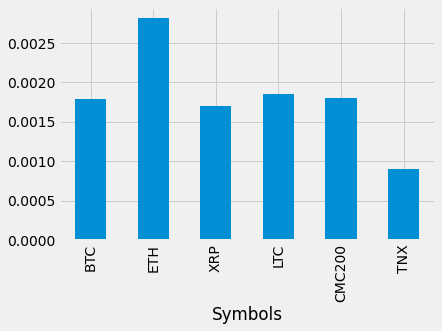
\includegraphics[height=5.8cm,keepaspectratio]{images/mean.png}
  \note{\textit{Note.} Own representation.}
\end{minipage}%
\begin{minipage}{.5\textwidth}
  \centering
  \caption{Standard deviations}
  \label{fig:std}
  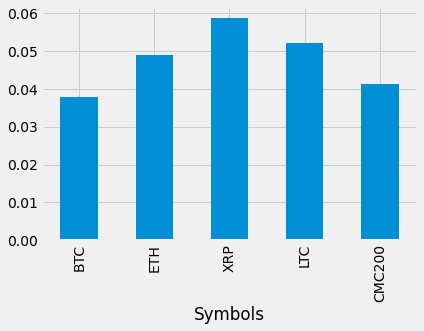
\includegraphics[height=5.8cm,keepaspectratio]{images/std.png}
  \note{\textit{Note.} Own representation.}
\end{minipage}
\end{figure}

Lastly, in Figure \ref{fig:mov_treasury} we tracked the price movement of the 10 year treasury yield and in Figure \ref{fig:mov_crypto} the price movement of the cryptocurrencies.

\begin{figure}
    \centering
    \caption{Covariance}
    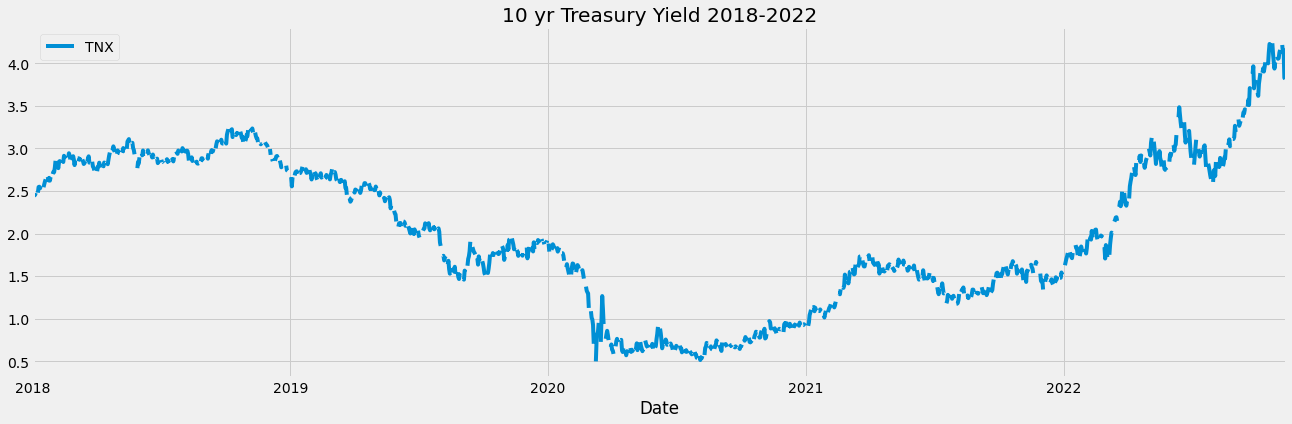
\includegraphics[width=\textwidth,height=\textheight,keepaspectratio]{images/movement_treasury.png}
    \label{fig:mov_treasury}
    \note{\textit{Note.} Own representation.}
\end{figure}

\begin{figure}
    \centering
    \caption{Covariance}
    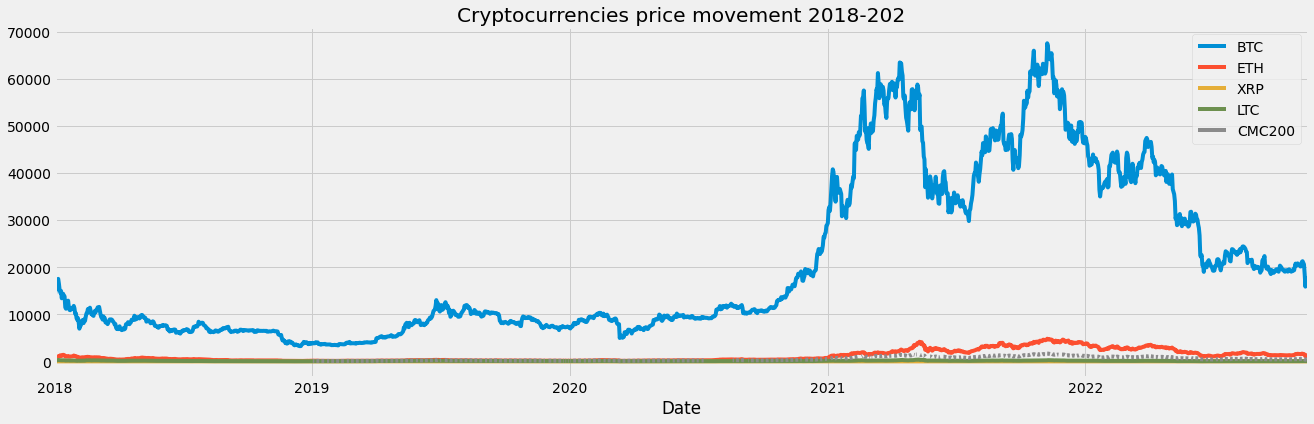
\includegraphics[width=\textwidth,height=\textheight,keepaspectratio]{images/movement_crypto.png}
    \label{fig:mov_crypto}
    \note{\textit{Note.} Own representation.}
\end{figure}